\documentclass[11pt,a4paper]{article}
\usepackage[T1]{fontenc}
\usepackage[margin=2.3cm]{geometry}
\usepackage{amsmath,amssymb}
\usepackage{graphicx}
\usepackage[dvipsnames]{xcolor}
\usepackage{enumitem}
\usepackage[colorlinks=true,linkcolor=blue,urlcolor=blue]{hyperref}
\setlength{\parskip}{0.6em}
\setlength{\parindent}{0pt}
\begin{document}

\begin{center}{\LARGE\bfseries opennowcast}\\[0.4em]{\large Nowcast rain by sliding the radar picture along the wind, in three sessions.}\\[0.2em]\small PAN IIT OSS explainer \textbullet{} secondary school to diploma / undergraduate (levels 3-5)\end{center}

\section*{Why this exists}
Short-range rain forecasts start from radar pictures. This explainer shows the mathematics behind moving a radar picture along its measured motion and measuring the result, using only shifts, interpolation and simple scores, so you can build it yourself.

\section*{The end goal}
Nowcast rain by advecting radar fields. The end goal is a rain nowcast made by advecting radar fields, as used in the first hour or two of operational forecasts: estimate the motion, move the rain, account for growth and uncertainty, and state honestly how far ahead the forecast can be trusted. This is a teaching model, not a weather warning system.

\section*{How the three sessions build up}
\begin{enumerate}[nosep]
\item \textbf{Session 1: A rain cell drifts with the wind} (Level 1, conceptual interactive model, 60 min).
\item \textbf{Session 2: Translate a field, estimate the motion, score the forecast} (Level 2, mathematical engineering model, 75 min).
\item \textbf{Session 3: When one shift is not enough: local motion, growth, uncertainty} (Level 3, simulation and validation, 90 min).
\end{enumerate}

\section{Session 1: A rain cell drifts with the wind}

\subsection*{A. Real-world problem}
A weather radar sends a new picture of rain every 5 minutes. In a picture a rain cell, a blob of heavy rain, is in one place; in the next picture it has moved. If we measure how far, we know the wind that carries it, and we can say when it will reach a town in the next hour. This is a nowcast: a forecast for the next hour or two. Safety note: this is a teaching model with made-up data. It is not a weather warning system. Always follow the official forecasts and warnings of your national weather service.

\subsection*{B. Concept and theory}
A radar picture is a grid of numbers. Here it is 100 x 100 pixels, one pixel is 1 km wide, and each pixel holds a rain rate in mm/h (millimetres of rain per hour). A rain cell is a smooth hill of rain: strongest at the centre and weaker outside, written as a Gaussian bell with centre rain rate P and width sigma. If the centre moved dx pixels east and dy pixels north in one 5 minute frame, the wind that carries it is 12 times those numbers in km/h, because 5 minutes is 1/12 of an hour and a pixel is 1 km. The key assumption of this whole repo: the wind stays the same during the forecast. Then the centre moves in a straight line at constant speed, and the rain at a town is the bell evaluated at the distance from the centre.

\begin{itemize}[nosep]
\item (x, y): position on the radar picture (km (1 pixel = 1 km))
\item R: rain rate (mm/h)
\item P: rain rate at the centre of the cell (40) (mm/h)
\item sigma: width of the cell (6) (km)
\item (u, v): wind carrying the cell, east and north (km/h)
\item d: distance from the cell centre to the town (km)
\item r: distance from the centre at which the rain falls to the threshold (km)
\end{itemize}

\begin{equation*}
R(d)=P\,\exp\!\left(-\frac{d^{2}}{2\sigma^{2}}\right)
\end{equation*}

\begin{equation*}
(u,v)=\frac{(\Delta x,\Delta y)\times 1\,\mathrm{km}}{5/60\ \mathrm{h}}=12\,(\Delta x,\Delta y)\ \mathrm{km/h}
\end{equation*}

\begin{equation*}
r=\sigma\sqrt{2\ln\!\left(P/R_{\mathrm{thr}}\right)}
\end{equation*}

\begin{equation*}
(x_c,y_c)(t)=(x_0,y_0)+(u,v)\,\frac{t}{60}\qquad(t\ \text{in minutes})
\end{equation*}

\begin{center}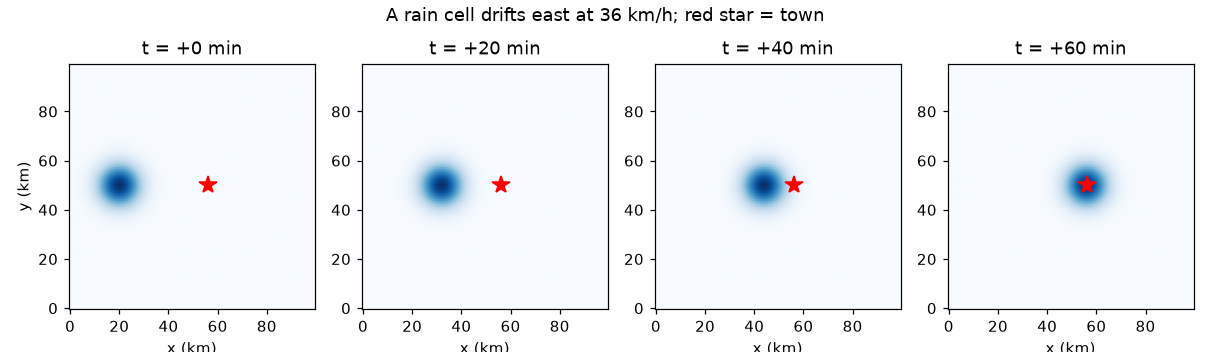
\includegraphics[width=0.85\linewidth]{figures/s01_drifting_cell.png}\\\small One cell drifting east at 36 km/h at 0, 20, 40 and 60 minutes; the red star is the town.\end{center}

\subsection*{E. Worked example}
Between two frames 5 minutes apart a cell (width 6 km, centre rain rate 40 mm/h) moved 3 pixels east. The town is 36 km east of the cell. What is the wind, when does the centre arrive, and when does the rain at the town first reach 5 mm/h?
\begin{enumerate}[nosep]
\item Wind = 12 x 3 = 36 km/h towards the east (3 km in 1/12 hour).
\item The centre arrives after 36 km / 36 km/h = 1 hour = 60 minutes.
\item The 5 mm/h edge of the cell is r = 6 x sqrt(2 ln(40/5)) = 6 x sqrt(2 x 2.079) = 12.24 km from the centre.
\item Rain of 5 mm/h reaches the town when the centre is 12.24 km away, that is after travelling 36 - 12.24 = 23.76 km, which takes 23.76 / 36 x 60 = 39.6 minutes.
\item Check: after 39.6 minutes the distance is 12.24 km and R = 40 exp(-12.24\textasciicircum{}2 / 72) = 5.0 mm/h.
\end{enumerate}
\textbf{Answer.} The wind is 36 km/h east, the centre arrives after 60 minutes, and rain of 5 mm/h or more starts after 39.6 minutes.

\subsection*{F. Questions}
\begin{enumerate}[nosep]
\item \textbf{Conceptual.} Why do we need two radar pictures to get the wind, and why do we assume the wind stays the same during the forecast?
\item \textbf{Numerical.} A cell moves 5 pixels east in 5 minutes. A town is 45 km east of its centre. What is the wind and when does the centre arrive?
\item \textbf{Graph and simulation interpretation.} In the graph of rain at the town, the wind straight at the town and the wind turned by 20 degrees give very different peaks. Read both peaks and explain the difference.
\item \textbf{Design and optimisation challenge.} Design: a town wants at least 20 minutes of warning before rain of 5 mm/h or more, for a cell moving straight at it at 36 km/h. How far away must the cell centre be at the moment the forecast is issued?
\end{enumerate}

\section{Session 2: Translate a field, estimate the motion, score the forecast}

\subsection*{A. Real-world problem}
A real nowcast moves the whole radar picture, not one cell. The motion is rarely a whole number of pixels, so we must shift by fractions of a pixel, and we must find the motion from two frames. Then comes the honest question: is the advected forecast any better than saying 'nothing changes' (persistence), and how do we measure that? A forecast that is displaced by a few kilometres looks bad pixel by pixel but may still be useful; good scores must take this into account. Safety note: synthetic data, teaching model only, not a warning system.

\subsection*{B. Concept and theory}
The field R(x, y) is a 100 x 100 array of rain rates. An integer shift copies the array to a new place (rain pushed off the edge is lost). For a shift by (dx, dy) that is not a whole number, the new value at a pixel is read from the old field at (x - dx, y - dy); that point lies between four pixels and we take a weighted average of them (bilinear interpolation). The four weights add up to 1, so total rain is conserved. Along one axis a fractional shift f uses the two weights (1 - f) and f; this averaging adds a blur of variance f(1 - f) pixels squared, which is largest (0.25) at f = 0.5. To estimate the motion we try shifts of the old frame and keep the one that makes the squared difference from the new frame smallest (the cousin of finding the peak of the cross-correlation), first in whole pixels, then on a finer grid. Persistence uses the latest frame as the forecast. Advection shifts it by (shift per frame) x (lead in frames). Skill: RMSE is the root mean squared difference (mm/h). CSI counts pixels at or above a threshold: hits / (hits + misses + false alarms). The fractions skill score (FSS) compares the fraction of rainy pixels in n x n windows, so it forgives small displacements. For a Gaussian cell the area above the threshold is a disc of radius r = sigma sqrt(2 ln(P/threshold)); two such discs displaced by d have CSI equal to overlap / union, which only depends on d / r. This explains why skill falls with lead time: d = (wind error) x (lead time).

\begin{itemize}[nosep]
\item R(x, y): rain rate field (mm/h)
\item (dx, dy): shift per frame, east and north (pixels per frame (1 pixel = 1 km))
\item f: fractional part of a shift (pixels)
\item thr: rain-rate threshold for CSI and FSS (5) (mm/h)
\item n: window size for FSS (pixels)
\item r: radius of the area above the threshold (km)
\item d: displacement between forecast and true cell (km)
\item e: error of the estimated wind (km/h)
\end{itemize}

\begin{equation*}
R'(x,y)=R(x-\Delta x,\;y-\Delta y)\quad\text{(bilinear weights }(1-f)\text{ and }f\text{ per axis)}
\end{equation*}

\begin{equation*}
\sigma^{2}_{\mathrm{added}}=f(1-f)\ \ \text{pixels}^2
\end{equation*}

\begin{equation*}
\mathrm{RMSE}=\sqrt{\frac{1}{N}\sum (F-O)^{2}},\qquad \mathrm{CSI}=\frac{H}{H+M+FA}
\end{equation*}

\begin{equation*}
\mathrm{FSS}=1-\frac{\overline{(P_F-P_O)^{2}}}{\overline{P_F^{2}}+\overline{P_O^{2}}}
\end{equation*}

\begin{equation*}
\mathrm{CSI}(d/r)=\frac{A_{\cap}}{2\pi r^{2}-A_{\cap}},\quad A_{\cap}=2r^{2}\arccos\frac{d}{2r}-\frac{d}{2}\sqrt{4r^{2}-d^{2}}
\end{equation*}

\begin{center}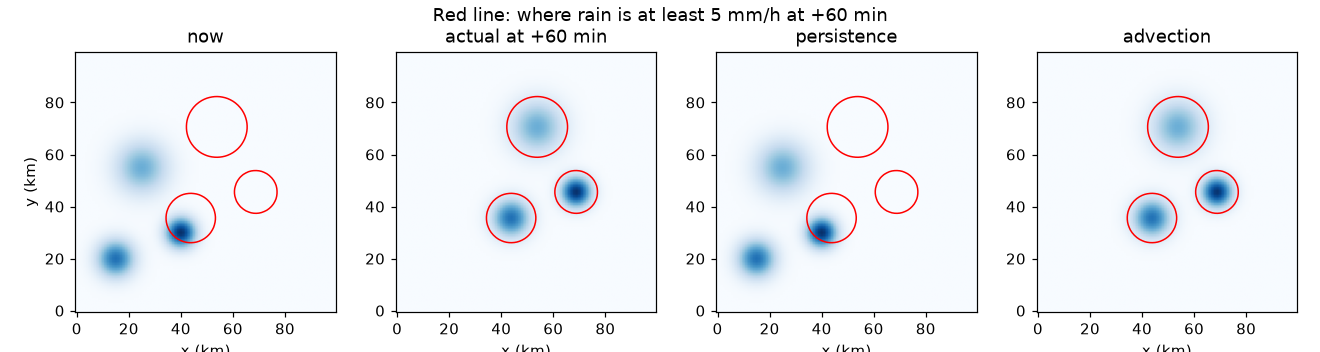
\includegraphics[width=0.85\linewidth]{figures/s02_forecast_panels.png}\\\small Now, truth at +60 minutes, persistence and advection; red outline marks 5 mm/h in the truth.\end{center}

\subsection*{E. Worked example}
Two frames show the whole pattern moved (2.4, 1.3) pixels in 5 minutes. What is the wind, how far does the pattern move in 60 minutes, and what is the CSI if a forecast has 80 hits, 10 misses and 10 false alarms?
\begin{enumerate}[nosep]
\item Wind: u = 2.4 x 12 = 28.8 km/h east and v = 1.3 x 12 = 15.6 km/h north.
\item Speed = sqrt(28.8\textasciicircum{}2 + 15.6\textasciicircum{}2) = sqrt(829.4 + 243.4) = 32.76 km/h.
\item In 60 minutes there are 12 frames, so the pattern moves (2.4 x 12, 1.3 x 12) = (28.8, 15.6) km.
\item CSI = hits / (hits + misses + false alarms) = 80 / (80 + 10 + 10) = 0.8.
\item Check with the code: \texttt{estimate\_shift} returns about (2.4, 1.3) and the checkpoint recomputes all of these.
\end{enumerate}
\textbf{Answer.} Wind (28.8, 15.6) km/h, speed 32.76 km/h; the pattern moves (28.8, 15.6) km in an hour; the CSI is 0.8.

\subsection*{F. Questions}
\begin{enumerate}[nosep]
\item \textbf{Conceptual.} Why does shifting a field by half a pixel make the peak lower, even though no rain is lost?
\item \textbf{Numerical.} The estimated shift is (1.5, 0.5) pixels per 5 minutes. Give the wind components and speed in km/h and the displacement after 60 minutes.
\item \textbf{Graph and simulation interpretation.} On the skill-against-lead-time graph for a translating field, which method wins and why does the other curve fall? Quote the 60 minute CSI values.
\item \textbf{Design and optimisation challenge.} Design: a cell has a 5 mm/h radius of 9.47 km. You want a CSI of at least 0.5 at 60 minutes. How accurate must the wind be? What if you only need 30 minutes?
\end{enumerate}

\section{Session 3: When one shift is not enough: local motion, growth, uncertainty}

\subsection*{A. Real-world problem}
Real storms do not move as one rigid sheet. One storm may move east while another, 60 km away, moves north-west. Cells also grow and fade, and the wind we measure is never exact. A forecaster would also like a probability ('how likely is 10 mm/h at my town?'), not only a single picture. In this session you build a local-motion nowcast, measure where it works and where it breaks, and finish with a mini-project. Safety note: synthetic data only; this is not a warning system. Real nowcasting is done by trained forecasters with validated systems.

\subsection*{B. Concept and theory}
Local motion: cut the picture into overlapping blocks (32 x 32 pixels, step 16). In each block that has rain, find the shift of the old frame that best matches the new frame inside the block (whole pixels, then a parabola fit for fractions). Empty blocks borrow the nearest vector; vectors are then interpolated to every pixel. Semi-Lagrangian advection: for every target pixel look back along the motion to where its rain came from and copy the value (interpolated); one look-back covers the whole lead time. Repeating small shifts instead interpolates at each step: with a fractional part f per step, n steps add n f (1 - f) pixels squared of blur, while one shift adds only f\_total (1 - f\_total). Growth: if a cell's peak changes by a factor (1 + g) per frame while advection keeps it constant, the area above the threshold is wrong; the radius of the area is r = sigma sqrt(2 ln(P (1 + g)\textasciicircum{}k / thr)) after k frames, and the CSI of two discs with different radii and a displacement d can be computed from circle overlap geometry. Uncertainty: add random errors to the wind (ensemble members), advect once per member and count the fraction of members with rain at or above the threshold; the Brier score (mean squared difference between probability and the 0/1 outcome) and a reliability table (forecast probability against observed frequency) judge the result. Advection cannot create rain: a storm that starts after the forecast time is invisible to it, and a rotating pattern has no single straight-line motion.

\begin{itemize}[nosep]
\item (u, v): motion vector (pixels per frame (1 pixel per 5 minutes = 12 km/h))
\item g: growth rate of the peak of a cell (per frame (0.08 = 8 \%))
\item k: lead time in frames (frames of 5 minutes)
\item thr: threshold for CSI (10) (mm/h)
\item r\_f, r\_t: radius of the forecast and true area above the threshold (km)
\item d: distance between their centres (km)
\item p: ensemble probability of rain at or above the threshold (0 to 1)
\item BS: Brier score (0 (best) to 1)
\end{itemize}

\begin{equation*}
\mathbf{x}_{\mathrm{dep}}=\mathbf{x}-k\,\mathbf{u}(\mathbf{x}_{\mathrm{dep}}),\qquad R_f(\mathbf{x})=R_0(\mathbf{x}_{\mathrm{dep}})
\end{equation*}

\begin{equation*}
n\,f(1-f)\ \text{(repeated steps)}\quad\text{versus}\quad f_{\mathrm{tot}}(1-f_{\mathrm{tot}})\ \text{(one shift)}
\end{equation*}

\begin{equation*}
r_t(k)=\sigma\sqrt{2\ln\!\left(\frac{P(1+g)^{k}}{\mathrm{thr}}\right)}
\end{equation*}

\begin{equation*}
\mathrm{BS}=\frac{1}{N}\sum_i (p_i-o_i)^{2}
\end{equation*}

\begin{center}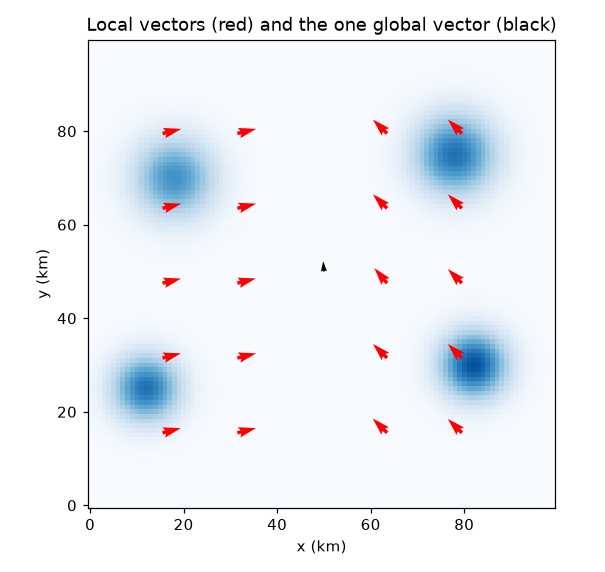
\includegraphics[width=0.85\linewidth]{figures/s03_motion_vectors.png}\\\small Local vectors (red) and the single global vector (black) on the two-region field.\end{center}

\subsection*{E. Worked example}
A cell of width sigma = 2.5 pixels moves 8.4 pixels east in 60 minutes (0.7 pixels per 5 minutes). Compare the blur from 12 separate 0.7 pixel shifts with one 8.4 pixel shift.
\begin{enumerate}[nosep]
\item One 0.7 pixel shift has fractional part f = 0.7 and adds f(1 - f) = 0.7 x 0.3 = 0.21 pixels squared of blur.
\item Twelve of them add 12 x 0.21 = 2.52 pixels squared.
\item One shift of 8.4 pixels has fractional part 0.4 and adds 0.4 x 0.6 = 0.24 pixels squared.
\item The cell starts with variance 6.25 pixels squared, so the 12-step cell is wider: its peak ends at 24.99 mm/h from 30, against 29.08 mm/h for the single shift.
\item Both conserve the total rain exactly; only the shape differs. The checkpoint measures all these numbers from the arrays.
\end{enumerate}
\textbf{Answer.} Twelve small interpolated steps add 2.52 pixels squared of blur and lower the peak to 24.99 mm/h; one 60-minute shift adds only 0.24 pixels squared and keeps 29.08 mm/h.

\subsection*{F. Questions}
\begin{enumerate}[nosep]
\item \textbf{Conceptual.} Why can advection never forecast a storm that starts after the forecast time? And why does a rotating pattern break a single-vector forecast?
\item \textbf{Numerical.} A cell is moved in 12 steps of 0.5 pixels. How much blur (in pixels squared) is added in total? How much would one shift of 6 pixels add?
\item \textbf{Graph and simulation interpretation.} In the growth and decay panel of the skill curves, at what lead time does each method fall below CSI 0.5 (10 mm/h)? What does that mean for a user?
\item \textbf{Design and optimisation challenge.} Design: you must publish a 60-minute forecast for a field with two regions that move differently and cells that grow and fade. Choose the motion method and the longest lead time you would show as a single picture, and say what you would show beyond that.
\end{enumerate}

\section{Real-world mini-project}
\textbf{Nowcast a two-region storm field for 60 minutes.} A synthetic radar scene (\texttt{GROWTH} in Session 3) has two regions that move differently, with cells that grow and fade. Make a nowcast from the last two frames with persistence, one global vector and local vectors, score each against the truth for every 5 minutes up to 60, and find the lead time at which each skill first drops below a CSI of 0.5. Repeat for the thresholds 5, 10 and 15 mm/h.

\section{The path ahead}
\begin{enumerate}[nosep]
\item \textbf{Session 4: Growth-aware advection.} A forecast that advects the field and multiplies it by a growth map that is itself advected.
\item \textbf{Session 5: Follow the rotation.} A forecast that advects in several sub-steps using the vectors at each new position.
\item \textbf{Session 6: Sharper long steps.} A stepping scheme that moves a cell for 60 minutes in 12 steps without smoothing it.
\item \textbf{Session 7: Reliable at every confidence level.} A probability forecast whose reliability table lies near the diagonal in every bin.
\item \textbf{Session 8: Storm initiation hints.} A rule that flags areas of likely initiation and a way to score it.
\end{enumerate}

\section{Answers and hints}

\subsection*{Session 1}
\begin{enumerate}[nosep]
\item \textbf{Conceptual.} Hint: One picture shows where the rain is, not where it is going. What do you need to measure a speed? Solution: A speed needs a distance and a time: the distance a cell moved between two pictures taken a known time apart. One picture has no motion information at all. The forecast then extends that motion into the future, which only works if the wind does not change; real winds change, which is why skill falls with lead time (Sessions 2 and 3).
\item \textbf{Numerical.} Hint: 12 km/h per pixel per frame; then time = distance / speed. Solution: Wind = 12 x 5 = 60 km/h. Time = 45 km / 60 km/h = 0.75 h = 45 minutes. Sanity check: 60 km/h is 1 km per minute, so 45 km takes 45 minutes.
\item \textbf{Graph and simulation interpretation.} Hint: Look at the miss distance and at how fast the bell falls away from the centre. Solution: The straight wind peaks at 40 mm/h (after 60 minutes). The turned wind peaks at only 4.87 mm/h, below the 5 mm/h line, after 56.4 minutes. The turned path passes 36 x sin(20 degrees) = 12.3 km from the town, and at 12.3 km the bell has fallen to 4.87 mm/h. The cell is narrow compared with the miss distance, so the direction matters a lot.
\item \textbf{Design and optimisation challenge.} Hint: 20 minutes of travel plus the distance from the centre to the 5 mm/h edge. Solution: In 20 minutes the cell moves 36 x 20/60 = 12 km. The rain reaches the town when the centre is 12.24 km away, so the centre must be 12 + 12.24 = 24.24 km away. Assumptions: constant wind and a cell that keeps its size. In practice add a safety margin because both are uncertain.
\end{enumerate}

\subsection*{Session 2}
\begin{enumerate}[nosep]
\item \textbf{Conceptual.} Hint: Each new value is a weighted average of neighbouring pixels. What does averaging do to a sharp peak? Solution: Bilinear interpolation averages neighbouring pixels. The weights add up to 1, so the total rain is unchanged, but a peak is averaged with its lower neighbours, so the peak falls and the cell spreads out. The added blur is f(1 - f) pixels squared per axis, largest at f = 0.5.
\item \textbf{Numerical.} Hint: Multiply by 12 for km/h; there are 12 frames in 60 minutes. Solution: u = 1.5 x 12 = 18 km/h and v = 0.5 x 12 = 6 km/h. Speed = sqrt(18\textasciicircum{}2 + 6\textasciicircum{}2) = sqrt(360) = 18.97 km/h. Displacement after 60 minutes = (18, 6) km. Sanity check: 18.97 km/h for one hour is about 19 km.
\item \textbf{Graph and simulation interpretation.} Hint: Persistence keeps the cells in the old place. Solution: Advection wins at every lead time. At 60 minutes its CSI is 0.996 against 0.074 for persistence. Persistence leaves the rain where it was while the true rain moved about 32 km, so the true and forecast areas almost do not overlap and CSI is close to zero. Advection moves the field with the right motion, so the overlap is nearly complete. This is the best case: constant wind, no growth.
\item \textbf{Design and optimisation challenge.} Hint: The two-disc model gives CSI 0.50 when d is about 5 km for r = 9.47 km. Displacement = wind error x time. Solution: At 60 minutes d = e x 1 h, so the wind error e must be at most about 5 km/h. At 30 minutes d = e x 0.5 h = 5 km needs e = 10 km/h, so the wind can be twice as bad. CSI depends only on d / r, so a cell twice as big tolerates twice the displacement. Trade-off: a forecast to a longer lead time needs a much more accurate wind; to a user, a larger scale answer (bigger area) is more reliable than a pixel-exact one.
\end{enumerate}

\subsection*{Session 3}
\begin{enumerate}[nosep]
\item \textbf{Conceptual.} Hint: What does advection do with the rain that is already in the picture? Solution: Advection only moves rain that already exists. A new storm has no rain in the latest picture, so it is missing from every forecast: in our test none of its 193 rainy pixels is forecast and the CSI falls from 0.90 to 0.72. A rotating pattern has no mean motion (the global vector is about zero), so global advection equals persistence, and even local straight-line vectors reach only a CSI of 0.08 at 60 minutes because the cells move on curved paths.
\item \textbf{Numerical.} Hint: Each step with fractional part f adds f(1 - f). Solution: Each step adds 0.5 x 0.5 = 0.25, so 12 steps add 3.0 pixels squared. A single shift of 6 pixels has fractional part 0, so it adds nothing. Same total movement, very different blur: this is why a nowcast should shift once by the total displacement.
\item \textbf{Graph and simulation interpretation.} Hint: Find where each curve crosses the dotted 0.5 line. Solution: Persistence falls below 0.5 at 10 minutes, the global vector at 15 minutes and local vectors at 45 minutes. A user relying on persistence or a single wind can trust the forecast for a quarter of an hour at most; local vectors give about 45 minutes. After that even the best method here is mostly wrong at 10 mm/h because cells grow and fade.
\item \textbf{Design and optimisation challenge.} Hint: Use the 0.5 crossing times for each method, and the reliability result. Solution: Use local vectors: a global vector falls below 0.5 at 15 minutes against 45 minutes for local vectors. Show the single picture up to about 45 minutes, where CSI at 10 mm/h stays above 0.5. Beyond that, show a probability map from an ensemble: the calibrated ensemble has a Brier score of 0.140 against 0.199 for a single answer, and its probabilities are reliable. Trade-off: local vectors are noisier in empty areas and cost more compute; a probability is harder for a user to read than a picture, so label it clearly. Always point users to official warnings.
\end{enumerate}

\section{How to join}
Read \texttt{CONTRIBUTING.md} in the repository, then pick an issue labelled \texttt{good first issue}. Repository: \url{https://github.com/KrunalPanchal1995/pan-iit-oss/tree/main/opennowcast}

\end{document}
